\section{Use case maps för konceptarkitektur}
\label{sec:use_case_koncept}

\begin{figure}[h]
    \centering
    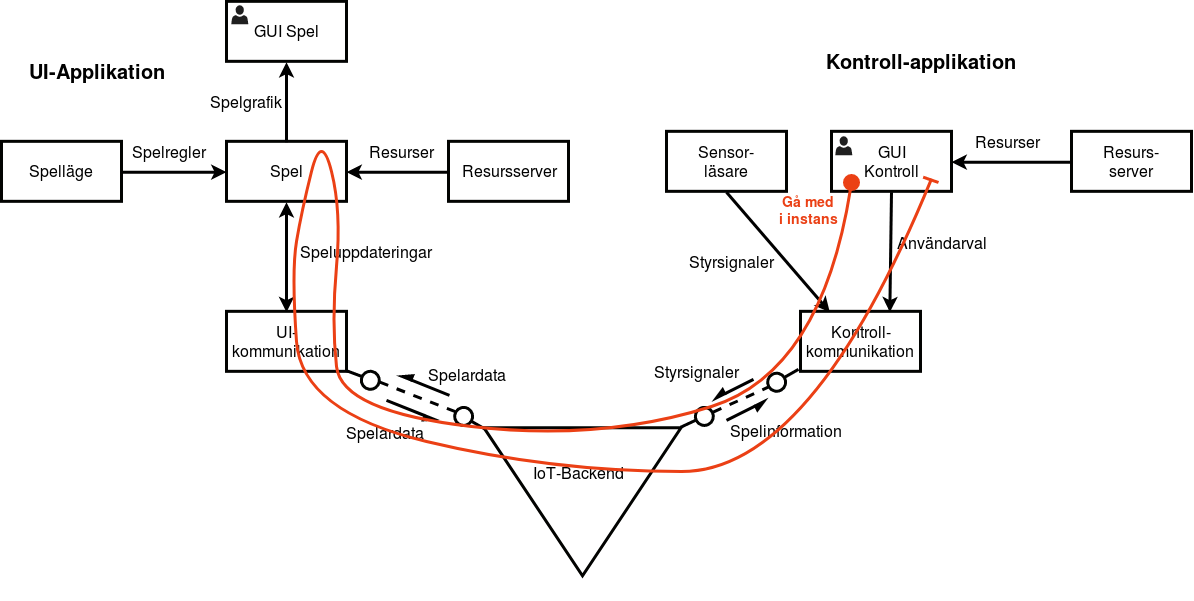
\includegraphics[scale=0.4]{konceptuell_use_case_join_instans}
    \caption{Use case map för att gå med i instans}
    \label{fig:use_case_koncept_join}
\end{figure}

\begin{figure}[h]
    \centering
    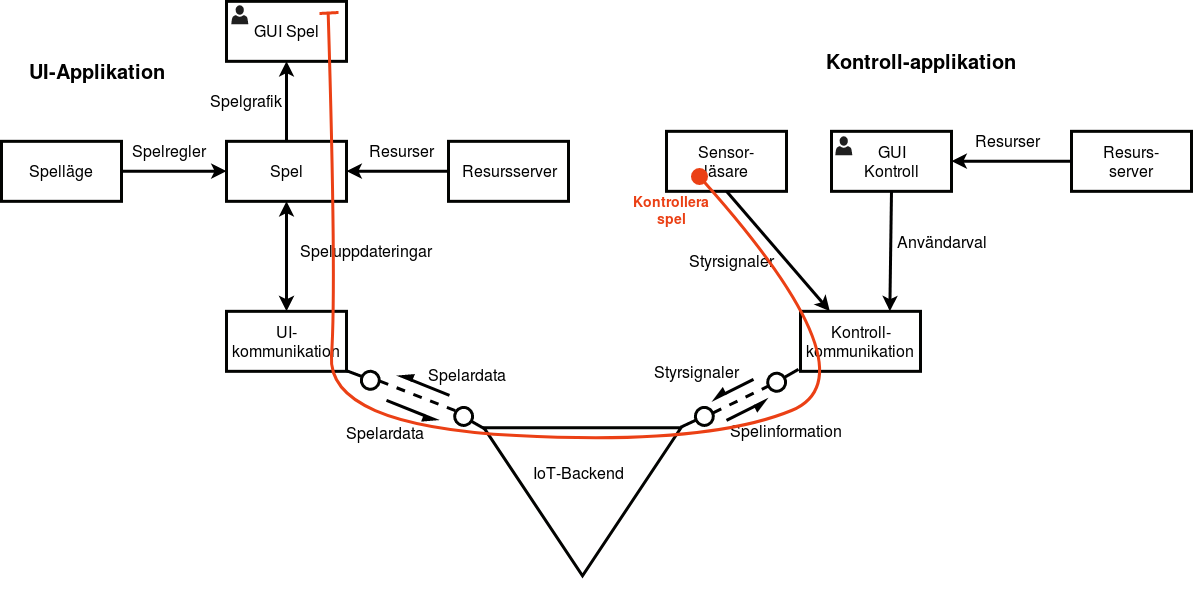
\includegraphics[scale=0.4]{konceptuell_use_case_kontrollera_spel}
    \caption{Use case map för att kontrollera spelet}
    \label{fig:use_case_koncept_kontrollera}
\end{figure}

\begin{figure}[h]
    \centering
    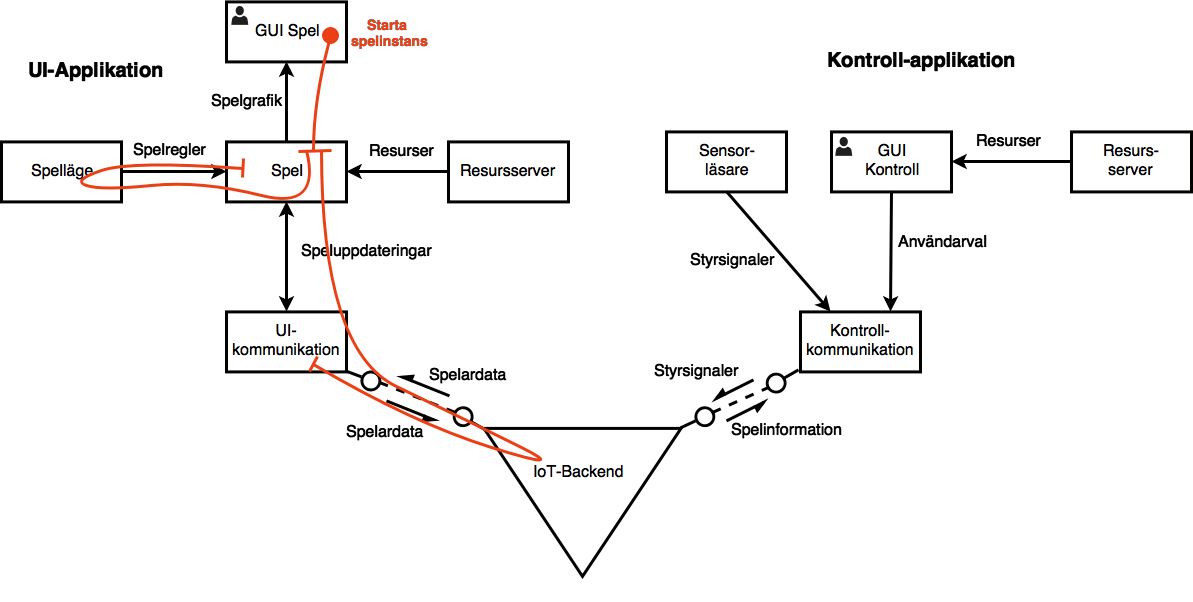
\includegraphics[scale=0.4]{konceptuell_use_case_starta_spelinstans}
    \caption{Use case map för att starta en spelinstans}
    \label{fig:use_case_koncept_starta_instans}
\end{figure}

\begin{figure}[h]
    \centering
    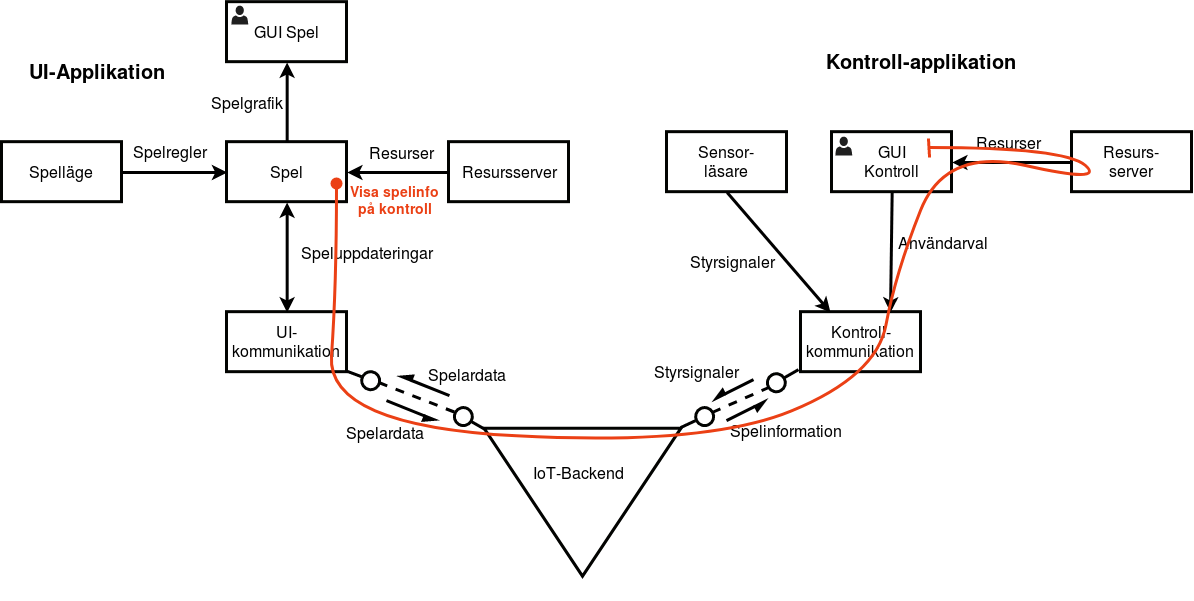
\includegraphics[scale=0.4]{images/konceptuell_use_case_visa_spelinfo}
    \caption{Use case map för att visa upp spelinformation i kontroll-applikationen}
    \label{fig:use_case_koncept_visa_spelinfo}
\end{figure}

\begin{figure}[h]
    \centering
    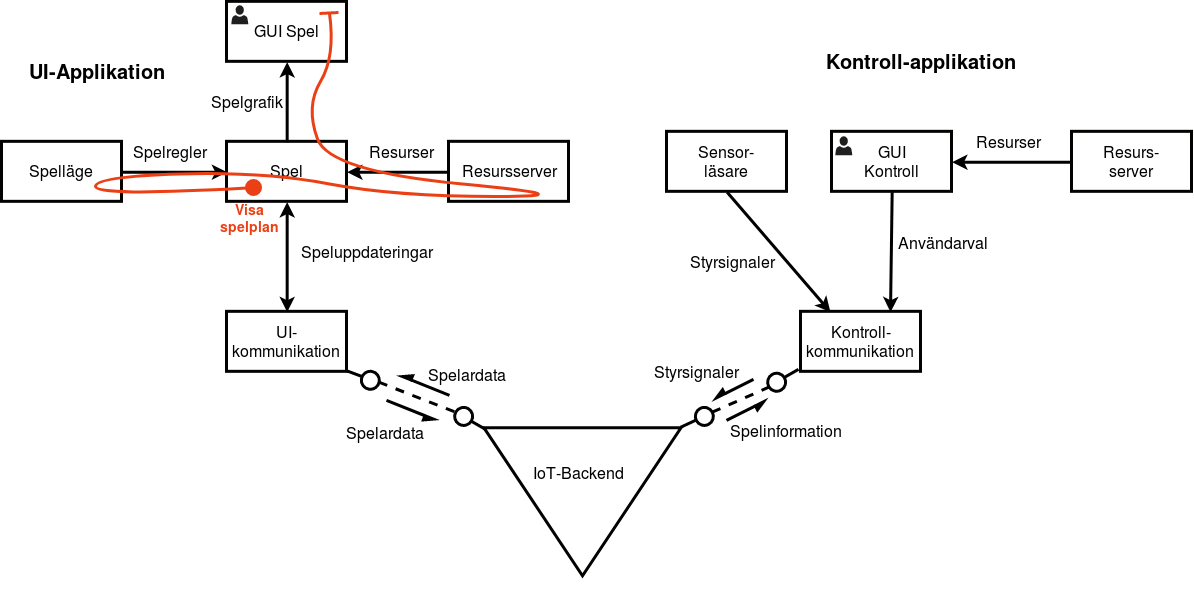
\includegraphics[scale=0.4]{images/konceptuell_use_case_visa_spelplan}
    \caption{Use case map för att visa upp spelplanen i UI-applikationen}
    \label{fig:use_case_koncept_visa_spelplan}
\end{figure}
